\chapter{Agentic Research Assistants、工具调用与验证边界}

\section{案例目标}

第 35 章讲的是：当 AI 帮你写出一段代码时，怎样通过验证回路判断它值不值得留下。本章再往前走一步，讨论另一个更现代的问题：\textbf{如果 AI 不只是给你一段代码，而是开始分步骤调用工具、读中间结果、再决定下一步呢？}

这时我们讨论的就不再只是“助手”，而是更接近\textbf{agentic workflow} 的结构。

本章的目标有三点：

\begin{enumerate}
    \item 理解什么叫 tool-using / agentic research assistant，以及它和单次回答式助手的差别；
    \item 理解为什么多步骤工作流必须有显式工具边界、停止条件和人工接管（human handoff）；
    \item 学会把一个极小的科研分诊任务拆成“质量门、novelty gate、评分、人工复核”四类步骤。
\end{enumerate}

\section{从“给我一个答案”到“按步骤完成任务”}

普通聊天式助手最常见的交互是：

\begin{itemize}
    \item 你提出一个问题；
    \item 它返回一段解释、代码或建议；
    \item 这一轮交互到此结束。
\end{itemize}

而 agentic workflow 的区别在于：模型不只输出一个最终文本，而是会在内部或显式地经历多个阶段，例如：

\begin{itemize}
    \item 先判断应该调用哪个工具；
    \item 再读取工具结果；
    \item 然后根据中间状态决定下一步；
    \item 最后把任务停在“完成”“失败”或“需要人工接管”的某个出口。
\end{itemize}

这类结构在科研里很有吸引力，因为很多工作流本来就是多步骤的：

\begin{itemize}
    \item 先做数据质量过滤，再做候选体排序；
    \item 先 cross-match，再判断 novelty；
    \item 先检查路径和 schema，再重构 notebook；
    \item 先跑 quick diagnostic，再决定是否需要更重的计算。
\end{itemize}

但它也更危险。因为一旦步骤变多，错误就可能以一种更隐蔽的方式传播：某个早期 gate 没跑、某个工具输出被误解、某个边界样本被代理强行拍板，最后都会让流程看起来非常流畅，却在科学上不可靠。

\section{一个极小的瞬变候选体分诊数据集}

配套 notebook 使用 \nolinkurl{transient_agent_workflow_demo.csv}。它是一个极小的教学版候选体表，每一行代表一个待分诊的 alert，包含：

\begin{itemize}
    \item \texttt{candidate\_id}；
    \item \texttt{alert\_score}；
    \item \texttt{rise\_rate\_mag\_day}；
    \item \texttt{color\_g\_r}；
    \item \texttt{crossmatch\_arcsec}；
    \item \texttt{image\_quality}；
    \item \texttt{moving\_object\_flag}；
    \item \texttt{reference\_action}。
\end{itemize}

这里的 \texttt{reference\_action} 不是“真理标签”，而是教学上预设的人类参考决策，分成三类：

\begin{itemize}
    \item \texttt{follow\_now}：可以直接进入高优先级 follow-up 队列；
    \item \texttt{manual\_review}：需要人工复核，不能由代理直接拍板；
    \item \texttt{reject}：应该被过滤或降级。
\end{itemize}

这个数据集故意放入了几类最容易让自动流程出错的样本：

\begin{itemize}
    \item \texttt{artifact} 图像质量但分数很高的候选体；
    \item 已知 moving object，但 alert 分数依然不低的候选体；
    \item 与已知源过近、novelty 证据不足的候选体；
    \item 边界分数样本，适合进入 \texttt{manual\_review} 而不是被强行二选一。
\end{itemize}

\section{先看一个单次排序 baseline}

如果不做任何多步骤流程，一个最常见的 baseline 就是：\textbf{只按 alert score 从高到低排序。}

\begin{examplebox}[单次排序 baseline]
\begin{lstlisting}[style=pythonstyle]
ranked = sorted(rows, key=lambda row: row["alert_score"], reverse=True)
top3 = ranked[:3]
\end{lstlisting}
\end{examplebox}

这种做法的问题非常直接：它把“最终优先级”当成了单一分数字段，而忽略了前面本应先执行的质量门和排除门。

在本章教学数据上，按 \texttt{alert\_score} 排名前三的对象里，会混入：

\begin{itemize}
    \item 一个 \texttt{artifact} 候选体；
    \item 一个已知 moving object；
    \item 只有一个真正应该 \texttt{follow\_now} 的候选体。
\end{itemize}

因此这个 baseline 的 top-3 precision 只有 \texttt{0.33}。

\begin{table}[htbp]
\centering
\small
\setlength{\tabcolsep}{4pt}
\begin{tabular}{@{}p{0.24\textwidth}>{\centering\arraybackslash}p{0.15\textwidth}>{\centering\arraybackslash}p{0.18\textwidth}p{0.26\textwidth}@{}}
\toprule
方法 & 直接 follow purity & 人工复核出口 & 教学解读 \\
\midrule
单次按 \texttt{alert\_score} 排序 & 0.33 & 否 & artifact 与 moving object 容易被推到前列 \\
显式工具链 workflow & 1.00 & 是 & 先过 gate，再评分，并保留 \texttt{manual\_review} \\
\bottomrule
\end{tabular}
\caption{本章 notebook 中两个最小流程的对照。重点不是“更像代理”，而是谁更尊重科研分诊的结构。}
\label{tab:ch36_baseline_vs_agentic}
\end{table}

\section{agentic workflow 的关键不是“能跑很多步”，而是“每一步做什么”}

本章 notebook 把流程拆成几类非常具体的工具步骤：

\begin{itemize}
    \item \textbf{artifact gate}：如果 \texttt{image\_quality == artifact}，直接拒绝；
    \item \textbf{moving-object gate}：如果 \texttt{moving\_object\_flag == yes}，直接拒绝；
    \item \textbf{novelty gate}：如果与已知源过近，就不能把它直接当成新瞬变；
    \item \textbf{priority score}：只对通过前面门的候选体做组合评分；
    \item \textbf{human handoff gate}：把边界样本送入 \texttt{manual\_review}。
\end{itemize}

最小形式可以写成：

\begin{examplebox}[一个最小 agentic routing 逻辑]
\begin{lstlisting}[style=pythonstyle]
if image_quality == "artifact":
    reject
elif moving_object_flag == "yes":
    reject
elif crossmatch_arcsec <= 0.8:
    reject
elif image_quality != "clean":
    manual_review
elif crossmatch_arcsec <= 1.5:
    manual_review
elif 0.58 <= score < 0.78:
    manual_review
elif score >= 0.78:
    follow_now
else:
    reject
\end{lstlisting}
\end{examplebox}

请注意，这里的“agentic”并不意味着模型在自由幻想。恰恰相反，它意味着你要把多步骤流程\textbf{收紧成一组明确的工具与出口}。

\section{为什么 human handoff 不是失败，而是正确出口}

很多初学者会误以为，一个“更强的代理”就应该尽量少把任务交回给人。但在科研里，这个直觉经常是错的。

如果一个候选体满足下面任一条件：

\begin{itemize}
    \item 图像质量不是完全 clean；
    \item novelty 支持不够强；
    \item 综合分数落在边界区间；
    \item 多个证据彼此冲突；
\end{itemize}

那么把它送进 \texttt{manual\_review} 往往不是“代理没能力”，而是\textbf{流程设计正确}。

这和第 35 章的验证回路逻辑是连续的：第 35 章强调“代码生成后要有回归检查”；本章则强调“多步骤代理运行时要有人工闸门”。两章本质上都在讲同一件事：\textbf{让 AI 在边界处停下来，而不是流畅地做错。}

图~\ref{fig:ch36_agentic_pipeline} 给出了本章 notebook 中的最小工具链。

\begin{figure}[htbp]
\centering
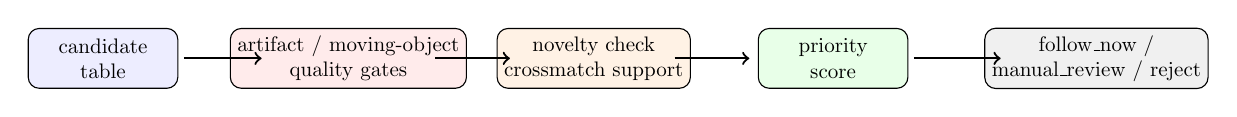
\begin{tikzpicture}[every node/.style={align=center}, scale=0.76, transform shape]
\node[draw, rounded corners, fill=blue!7, minimum width=2.5cm, minimum height=1.0cm] at (0,0) (load) {candidate\\table};
\node[draw, rounded corners, fill=red!8, minimum width=2.8cm, minimum height=1.0cm] at (4.1,0) (gates) {artifact / moving-object\\quality gates};
\node[draw, rounded corners, fill=orange!10, minimum width=2.7cm, minimum height=1.0cm] at (8.2,0) (novelty) {novelty check\\crossmatch support};
\node[draw, rounded corners, fill=green!9, minimum width=2.5cm, minimum height=1.0cm] at (12.2,0) (score) {priority\\score};
\node[draw, rounded corners, fill=gray!12, minimum width=3.0cm, minimum height=1.0cm] at (16.6,0) (exit) {follow\_now /\\manual\_review / reject};

\draw[->, thick] (1.35,0) -- (2.65,0);
\draw[->, thick] (5.55,0) -- (6.8,0);
\draw[->, thick] (9.55,0) -- (10.8,0);
\draw[->, thick] (13.55,0) -- (15.0,0);
\end{tikzpicture}
\caption{最小多步工具链示意图。}
\label{fig:ch36_agentic_pipeline}
\end{figure}

\section{notebook 如何把代理流程变成可审计记录}

在教学 notebook 里，我们故意不直接接任何真实在线 agent 框架，而是把流程写成清楚的函数和日志：

\begin{itemize}
    \item 用 \texttt{followup\_score()} 显式计算评分；
    \item 用 \texttt{route\_candidate()} 显式决定出口；
    \item 用 \texttt{run\_agentic\_triage()} 生成每个候选体的 action log；
    \item 最后再输出 confusion matrix、follow-now purity 和 manual-review 队列。
\end{itemize}

这样做的好处有三个：

\begin{itemize}
    \item notebook smoke test 可以直接运行；
    \item 每个中间状态都能被打印和检查；
    \item 将来如果你真要换成真实代理框架，也知道\textbf{应该保留哪些可见结构}。
\end{itemize}

也就是说，真正要迁移的不是某个 API 名字，而是流程设计：

\begin{itemize}
    \item 工具清单是否明确；
    \item 执行顺序是否合理；
    \item 停止条件是否可写清；
    \item 人工接管出口是否存在。
\end{itemize}

\section{一个更适合 agentic workflow 的 prompt 结构}

当任务变成多步骤流程时，prompt 也不应该只写“帮我排个序”。更好的做法是明确说明：

\begin{itemize}
    \item 候选表有哪些字段；
    \item 哪些 gate 必须先于排序执行；
    \item 哪些情况必须停在人工复核；
    \item 你希望代理输出的是工具顺序、停止条件还是最终队列。
\end{itemize}

\begin{examplebox}[一个更适合多步骤科研代理的 prompt 模板]
\begin{lstlisting}[style=pythonstyle]
prompt = """
你是我的科研工作流助手。

任务：
1. 先阅读候选体表的列定义；
2. 明确哪些工具步骤必须先于排序执行；
3. 给出 stop conditions 和 human handoff 条件；
4. 最后输出一个 follow-now 队列和一个 manual-review 队列。

流程约束：
- artifact 和 moving_object 不能直接进入高优先级列表
- novelty 支持不足的样本应进入人工复核
- 排序之前必须先跑质量门和 novelty gate
"""
\end{lstlisting}
\end{examplebox}

这里最关键的，不是某个华丽的措辞，而是你是否把“工具顺序”和“停止条件”说清楚。只要这些边界没讲明白，代理就很可能在一个不该自动化的地方擅自继续。

\section{配套 notebook 做了什么}

本章 notebook 的最小结构如下：

\begin{itemize}
    \item 先读取瞬变候选体表，并打印字段统计；
    \item 用单次 \texttt{alert\_score} 排序做 baseline；
    \item 再实现一个最小 tool-using agentic workflow；
    \item 输出 action log、最终队列和与参考决策的一致性；
    \item 最后打印一个适合多步骤代理的 prompt 模板与 workflow checklist。
\end{itemize}

它的重点不是追求“拟真大代理”，而是让学生先理解：\textbf{在科研里，多步骤代理真正需要设计的是结构，而不是神秘感。}

\section{和第 35 章、以及 Capstone 的关系}

可以把第 35 章和本章连起来理解：

\begin{itemize}
    \item 第 35 章解决的是“一段 AI 生成代码如何验证”；
    \item 本章解决的是“一个 AI 多步骤流程怎样被约束和审计”；
    \item 两章共同回答的，其实都是“怎样把 AI 放进科研工作流而不让它失控”。
\end{itemize}

到了 Capstone 阶段，这种能力会变得更加重要。真实项目里，你很可能会让 AI 帮你：

\begin{itemize}
    \item 整理候选体表；
    \item 执行一串数据检查与 cross-match；
    \item 组织 follow-up 队列；
    \item 把边界样本总结成给导师或组会使用的 review note。
\end{itemize}

但这些事情能不能安全地自动化，不取决于代理“像不像智能体”，而取决于你有没有把工具边界、行动日志、停止条件和人工复核出口预先设计好。

在最终 capstone 包里，action log 会成为 Integrity card 的一部分，manual review queue 会进入 Evaluation / Interpretation cards。它们共同回答一个问题：代理每一步为什么这样做，以及它在哪些边界处停下来交还给人。

\begin{warnbox}[科研代理 workflow 中的常见误区]
\begin{itemize}
    \item 让代理直接输出最终队列，却不保留中间工具步骤；
    \item 把排序分数当成唯一判断，跳过质量门与 novelty gate；
    \item 把 \texttt{manual\_review} 视为失败，而不是必要出口；
    \item 不记录 action log，导致后续无法追踪代理为什么这么做；
    \item 以为“更多步”天然更智能，忽略多步骤也会放大错误传播。
\end{itemize}
\end{warnbox}

\section{AI 助手如何帮助你}

在这个案例里，AI 助手最适合帮助你：

\begin{itemize}
    \item 帮你把多步骤工作流拆成更清楚的函数和工具接口；
    \item 帮你检查哪些 gate 应该先于排序执行；
    \item 帮你把人工接管条件写成明确、可审计的规则；
    \item 帮你整理 action log、review queue 和报告文字；
    \item 帮你比较“一次性回答”和“多步骤代理”两种 workflow 的风险差异。
\end{itemize}

但最终哪些样本值得自动 follow、哪些必须人工复核、以及哪些工具调用顺序符合你的科学目标，仍然需要你自己判断。

\section{练习}

\begin{exercisebox}[基础练习]
把教学数据里某一个 \texttt{manual\_review} 样本的 \texttt{image\_quality} 从 \texttt{clean} 改成 \texttt{artifact}，重新运行 notebook，观察 action log 和最终队列怎样变化。
\end{exercisebox}

\begin{exercisebox}[进阶练习]
请为本章 notebook 增加一个“最大步骤数”限制，并在 action log 里记录代理是否因为达到 step budget 而被迫停止。思考这和真实 agent 系统中的 loop control 有什么关系。
\end{exercisebox}

\begin{exercisebox}[开放练习]
结合第 35 章，设计一个你自己的科研代理规范：至少包括工具白名单、允许自动执行的步骤、必须人工确认的节点、以及需要固定在实验记录里的日志字段。
\end{exercisebox}

\section{本章小结}

本章最重要的结论是：\textbf{agentic research assistant 的价值，不在于让模型无限制地自己做决定，而在于把一个多步骤科研任务拆成有限、可见、可审计的工具链，并在边界处正确地停下来。} 只有这样，AI 才是在帮助你的工作流，而不是把错误更流畅地自动化。
